% !TeX root = ../main.tex

\chapter{神经网络模型嵌入 FFmpeg}

\section{环境搭建}

环境为 ubuntu-20.04,机器配置为 nvidia-460+cuda-11.2,FFmpeg 版本为 4.3.1。LibTorch 版本为 1.7.1+cu110。
如图 \ref{fig:myplay} 所示,FFmpeg 提供库文件和头文件,LibTorch 提供 Torch 的 C++ 前端 API。nvidia 驱动和 cuda 则提供 GPU 加速环境。

\subsection{通过源码安装FFmpeg-4.3.1}

\subsubsection{安装依赖库}

安装SDL2。ffplay依赖SDL,如果没有SDL,将不会编译产生可执行文件ffplay。SDL2可以下载源码编译安装,也可以通过包管理工具apt安装(推荐)。

\begin{lstlisting}
sudo apt install libsdl2-dev
\end{lstlisting}

安装yasm。yasm 用于对汇编优化的支持,若不需要汇编优化的支持,可在编译选项中关闭yasm即可(–disable-yasm)。

\begin{lstlisting}
sudo apt install yasm
\end{lstlisting}

\subsubsection{安装FFmpeg}

下载ffmpeg-4.3.1源码并解压。

\begin{lstlisting}
wget http://ffmpeg.org/releases/ffmpeg-4.3.1.tar.gz
tar zxf ffmpeg-4.3.1.tar.gz
\end{lstlisting}

为了不污染源码,在根目录下新建build文件夹,在里面执行configure和make操作。--enable-shared是为了生成so动态库。这里的
build文件夹下会生成一些config头文件,这是源码里没有的。这些头文件在后面单独编译ffplay源码时会用得到。

\begin{lstlisting}
cd ffmpeg-4.3.1
mkdir build && cd build
./../configure --prefix=/usr/local/ffmpeg --enable-shared
make
sudo make install
\end{lstlisting}

然后使用vim修改环境变量。

\begin{lstlisting}
// 打开配置文件
vim ~/.bashrc
// 在文件末尾添加
export PATH=/usr/local/ffmpeg/bin:$PATH
export LIBRARY_PATH=/usr/local/ffmpeg/lib:$LIBRARY_PATH
export LD_LIBRARY_PATH=/usr/local/ffmpeg/lib:$LD_LIBRARY_PATH
// 使配置文件生效
source ~/.bashrc
\end{lstlisting}

测试是否安装成功。

\begin{lstlisting}
ffmpeg -version
ffplay -version
\end{lstlisting}

\subsection{安装nvidia-460和cuda-11.2}

配置GPU加速环境,可以参考 \url{https://blog.csdn.net/weixin_43742643/article/details/115355545},安装过程不予详述。

\subsection{安装 libtorch}

libtorch是pytorch的C++前端,官网提供了编译好的最新版本。我也总结了一份所有版本的集合,地址为 
\url{https://blog.csdn.net/weixin_43742643/article/details/114156298}
。需要注意的是,libtorch 在 1.5.0 版本之前使用 CXX 11 标准编译,从 1.5.0 版本
开始使用 CXX 14 标准编译。这里选择下载 libtorch-1.7.1 的 cu110 版本

\begin{lstlisting}
wget https://download.pytorch.org/libtorch/cu110/libtorch-shared-with-deps-1.7.1%2Bcu110.zip
unzip libtorch-shared-with-deps-1.7.1%2Bcu110.zip
mv libtorch libtorch-1.7.1
\end{lstlisting}

\section{单独编译ffplay}

CMake是一个跨平台的开源工具,用于构建,测试和打包项目,CMake使用独立于编译器的配置文件来控制项目的编译过程,可以生成
makefile文件。pytorch官网推荐使用cmake工具对C++前端项目进行管理。值得注意的是,ffplay源码是用C
语言写的,但是需要在其中加入C++前端模型,因此需要将源码文件ffplay.c改为ffplay.cpp。

\subsection{创建工程}

首先,创建根目录MYPLAY-ROOT,其目录结构如下所示。其中CMakeLists.txt即为cmake配置文件,其余三个
文件均来自源码 ffmpeg-4.3.1/fftools/ 文件夹下。

\begin{lstlisting}
.
├── CMakeLists.txt
├── cmdutils.c
├── cmdutils.h
└── ffplay.cpp
\end{lstlisting}

\subsection{编辑CMakeLists.txt}

libtorch作为第三方库需要手动添加。使用PATHS关键字指定路径。

\begin{lstlisting}
find_package(Torch REQUIRED PATHS ~/libtorch-1.7.1)
\end{lstlisting}

ffplay源码提供了主要的头文件,build文件夹则提供了一些编译以后生成的config头文件。

\begin{lstlisting}
set(FFMPEG_SOURCE ~/ffmpeg-4.3.1)
include_directories(${FFMPEG_SOURCE})
set(FFMPEG_BUILD ~/ffmpeg-4.3.1/build)
include_directories(${FFMPEG_BUILD})
\end{lstlisting}

添加编译选项 -fpermissive 是因为 ffplay.c 转为 cpp 文件后会严格检查类型转换,导致出现大量
error,该选项可以把此类 error 降为 warning。

\begin{lstlisting}
set(CMAKE_CXX_FLAGS   "-fpermissive -w -g")
\end{lstlisting}

编译可执行文件时链接ffmpeg动态库

\begin{lstlisting}
target_link_libraries(myplay ${TORCH_LIBRARIES} -lavcodec -lavdevice -lavfilter -lavformat -lavutil -lswresample -lswscale -lm -lSDL2
)
\end{lstlisting}

使用CXX 14标准进行编译

\begin{lstlisting}
set_property(TARGET myplay PROPERTY CXX_STANDARD 14)
\end{lstlisting}

\subsection{修改cmdutils.h}

定位到 249 行,这个函数的形参和 C++ 关键字 class 重名,把形参 class 改成 myclass 即可。

\begin{lstlisting}
# 修改前
void show_help_children(const AVClass *class, int flags);
# 修改后
void show_help_children(const AVClass *myclass, int flags);
\end{lstlisting}

\subsection{修改ffplay.cpp}

首先增加Torch头文件

\begin{lstlisting}
#include <torch/torch.h>
#include <torch/script.h>
\end{lstlisting}

ffmpeg 是用 C 写的,由于现在是 cpp 文件,需要将与 ffmpeg 相关的头文件使用关键字
extern C {} 包裹。头文件cmdutils.h也要包裹进去。

\begin{lstlisting}
#include "libavutil/avstring.h"
#include "libavutil/eval.h"
#include "libavutil/mathematics.h"
#include "libavutil/pixdesc.h"
#include "libavutil/imgutils.h"
#include "libavutil/dict.h"
#include "libavutil/parseutils.h"
#include "libavutil/samplefmt.h"
#include "libavutil/avassert.h"
#include "libavutil/time.h"
#include "libavutil/bprint.h"
#include "libavformat/avformat.h"
#include "libavdevice/avdevice.h"
#include "libswscale/swscale.h"
#include "libavutil/opt.h"
#include "libavcodec/avfft.h"
#include "libswresample/swresample.h"

#if CONFIG_AVFILTER
# include "libavfilter/avfilter.h"
# include "libavfilter/buffersink.h"
# include "libavfilter/buffersrc.h"
#endif

#include "cmdutils.h"
}
\end{lstlisting}

枚举类型 SHOW\_MODE 定义在结构体 VideoState 内部,由于现在是 cpp 文件,使用时需要加上前缀
VideoState::ShowMode:: 。为了方便起见,直接添加宏定义如下(位置必须放在结构体 VideoState 定
义之后):

\begin{lstlisting}
#define ShowMode VideoState::ShowMode
#define SHOW_MODE_NONE ShowMode::SHOW_MODE_NONE
#define SHOW_MODE_VIDEO ShowMode::SHOW_MODE_VIDEO
#define SHOW_MODE_WAVES ShowMode::SHOW_MODE_WAVES
#define SHOW_MODE_RDFT ShowMode::SHOW_MODE_RDFT
#define SHOW_MODE_NB ShowMode::SHOW_MODE_NB
\end{lstlisting}

定位到函数 opt\_show\_mode(),其内部调用的函数 parse\_number\_or\_die() 的返回值是 double 类型,C++无法将其
转化为VideoState::ShowMode 枚举类型。但C++是可以把整形识别为枚举类型的,因此可以强制类型转换把double转为int。

\begin{lstlisting}
show_mode = !strcmp(arg, "video") ? SHOW_MODE_VIDEO :
    !strcmp(arg, "waves") ? SHOW_MODE_WAVES :
    !strcmp(arg, "rdft" ) ? SHOW_MODE_RDFT :
    (int)parse_number_or_die(opt, arg, OPT_INT, 0, SHOW_MODE_NB-1);
\end{lstlisting}

\section{在ffplay中嵌入模型}

这部分的主要内容是介绍将神经网络模型嵌入到 ffplay.cpp 中。
ffplay 把视频分解为帧,每一帧的处理都在 video\_image\_display() 函数中,该函数又调用
upload\_texture() 将帧的像素数据更新到纹理。如图 \ref{fig:flow} 所示,可以在 upload\_texture() 函数中调用神经网络模型,对帧画面进行处理,
神经网络模型的初试化则可以放在 main() 中。

\begin{figure}[h]
\centering
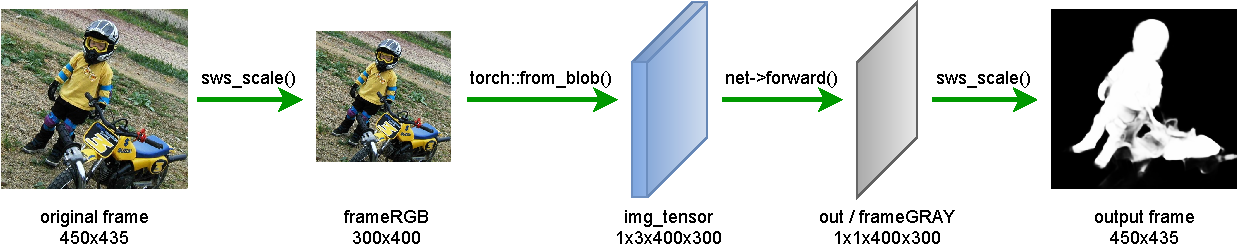
\includegraphics[width=1\textwidth]{flow.pdf}
\caption{帧数据处理过程}
\label{fig:flow}
% \note{注:图注的内容不宜放到图题中。}
\end{figure}

\subsection{神经网络模型初始化}

神经网络模型的初始化在 main() 中完成,这里介绍两种方式,见图 \ref{fig:twoways}。
第一种是用 TorchScript 工具导出模型 poolnet.pt,模型中不仅包含各参数的值,还包括神经网络各层的结构,因此可以直接在C++中生成神经网络。
第二种是使用C++前端API重新构建神经网络类,然后把类对象实例化,不过其参数权重依旧从 poolnet.pt 中导入。这种方法工程量相对较多。

\begin{figure}[h]
\centering
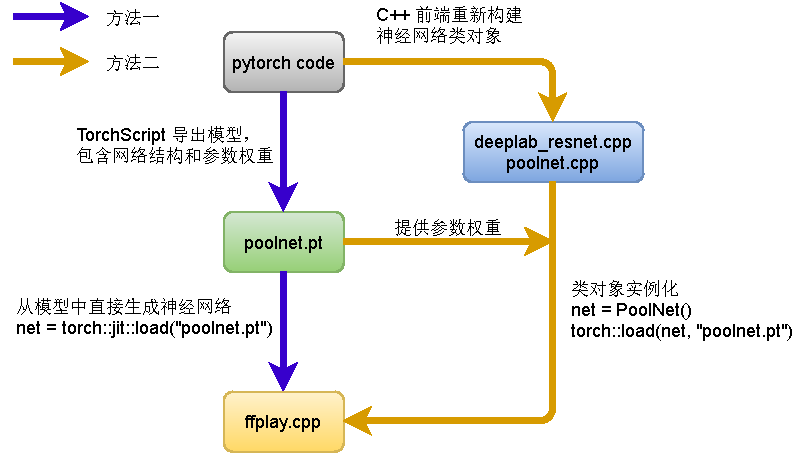
\includegraphics[width=1\textwidth]{twoways.pdf}
\caption{在ffplay中嵌入模型}
\label{fig:twoways}
% \note{注:图注的内容不宜放到图题中。}
\end{figure}

\subsubsection{从参数模型导入神经网络}

使用 jit::load 直接从参数模型 poolnet.pt 中导入神经网络。

\begin{lstlisting}
net = torch::jit::load("../models/poolnet.pt");
net.to(torch::kCUDA);
net.eval();
\end{lstlisting}

\subsubsection{神经网络类实例化}

PoolNet() 是使用Torch的C++前端API复现的神经网络类。通过 load 可以加载训练好的参数模型。

\begin{lstlisting}
net = PoolNet();
torch::load(net, "../models/poolnet.pt");
net->to(torch::kCUDA);
net->eval();
\end{lstlisting}

\subsection{原始帧数据转为RGB格式}

视频帧的格式一般为YUV格式,而神经网络模型的输入一般为三通道的RGB数据,因此,需要将原始帧数据转为RGB格式。frameRGB的类型是
AVFrame *,是帧指针,使用 av\_frame\_alloc() 进行初始化。frameRGB的宽和高应满足神经网络模型的要求,其格式为RGB。buffer申请
的空间用于frameRGB存储数据。这样即完成了RGB帧的构建。

\begin{lstlisting}
frameRGB = av_frame_alloc();
frameRGB->width = input_image_size;
frameRGB->height = input_image_size;
frameRGB->format = AV_PIX_FMT_RGB24;
numBytes = avpicture_get_size(frameRGB->format, frameRGB->width, frameRGB->height);
buffer = (uint8_t *)av_malloc(numBytes*sizeof(uint8_t));
avpicture_fill((AVPicture *)frameRGB, buffer, frameRGB->format, frameRGB->width, frameRGB->height);
\end{lstlisting}

frame是原始帧,frameRGB帧用来存储转换结果,*img\_convert\_ctx 用来存储转换前后的相关信息。sws\_scale() 函数则负责转换。

\begin{lstlisting}
*img_convert_ctx = sws_getCachedContext(*img_convert_ctx,
    frame->width, frame->height, frame->format, 
    frameRGB->width, frameRGB->height, frameRGB->format, 
    sws_flags, NULL, NULL, NULL);
if (*img_convert_ctx != NULL) {
    uint8_t *pixels[4];
    int pitch[4];
    if (!SDL_LockTexture(*tex, NULL, (void **)pixels, pitch)) {
        sws_scale(*img_convert_ctx, (const uint8_t * const *)frame->data, frame->linesize,
            0, frame->height, frameRGB->data, frameRGB->linesize);
        SDL_UnlockTexture(*tex);
    }
}
\end{lstlisting}

\subsection{从RGB帧中读取数据}

frameRGB->data[0] 为帧数据首地址,from\_blob() 函数可以从外部内存创建一个张量。premute() 用于调整张量形状为 
\{1,3,frameRGB->height,frameRGB->width\},toType() 再把类型转为float。

\begin{lstlisting}
torch::Tensor img_tensor = torch::from_blob(frameRGB->data[0], {1, frameRGB->height, frameRGB->width, 3}, torch::kByte).to(torch::kCUDA);
img_tensor = img_tensor.permute({0,3,1,2}).toType(torch::kFloat);
\end{lstlisting}

\subsection{利用神经网络进行推理}

如果神经网络是从参数模型导入,

\begin{lstlisting}
torch::Tensor out = net.forward({img_tensor}).toTensor();
\end{lstlisting}

如果神经网络是从类对象构造,

\begin{lstlisting}
torch::Tensor out = net->forward(img_tensor);
\end{lstlisting}

\subsection{处理输出结果}

out 的形状是 \{1,1,frameRGB->height,frameRGB->width\},需要转化为 \{frameRGB->height,frameRGB->width\}。to(torch::kCPU) 负责把张量从
GPU 转移到 CPU 上。

\begin{lstlisting}
out = out.squeeze().sigmoid().mul(255.0).toType(torch::kByte).to(torch::kCPU);
\end{lstlisting}

\subsection{将结果转换到原始帧中}

out.data\_ptr() 是张量数据的首地址,memcpy() 将数据从张量复制到frameRGB帧,然后再通过 sws\_scale() 转换为原始帧的大小和格式。

\begin{lstlisting}
auto frameGRAY = out;
int frameGRAY_width = frameRGB->width;
int frameGRAY_height = frameRGB->height;
*img_convert_ctx = sws_getCachedContext(*img_convert_ctx,
    frameGRAY_width, frameGRAY_height, AV_PIX_FMT_GRAY8, 
    frame->width, frame->height, frame->format, 
    sws_flags, NULL, NULL, NULL);
if (*img_convert_ctx != NULL) {
    uint8_t *pixels[4], *frameGRAY_data[8];
    int pitch[4], frameGARY_linesize[8];
    frameGRAY_data[0] = out.data_ptr();
    frameGARY_linesize[0] = frameGRAY_width;
    if (!SDL_LockTexture(*tex, NULL, (void **)pixels, pitch)) {
        sws_scale(*img_convert_ctx, (const uint8_t * const *)frameGRAY_data, frameGARY_linesize,
            0, frameGRAY_height, frame->data, frame->linesize);
        SDL_UnlockTexture(*tex);
    }
}
\end{lstlisting}

\subsection{运行}

新建目录 MYPLAY-ROOT/build,执行

\begin{lstlisting}
cmake ..
make
myplay -v quiet ../videos/test.gif
\end{lstlisting}

运行结果如图 \ref{fig:show} 所示

\begin{figure}[h]
\centering
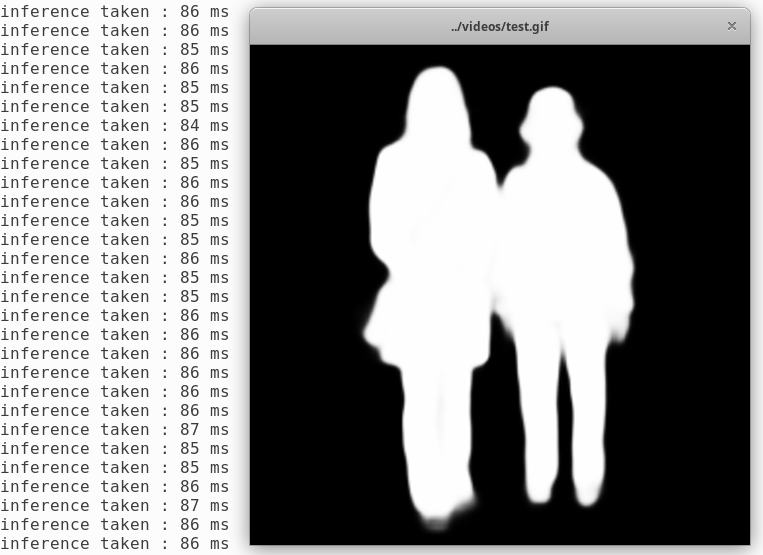
\includegraphics[width=0.8\textwidth]{show.PNG}
\caption{运行结果}
\label{fig:show}
% \note{注:图注的内容不宜放到图题中。}
\end{figure}